\documentclass{article}
\usepackage[utf8]{inputenc}
\usepackage{hyperref}
\usepackage{amsmath,amssymb}
\usepackage{mathtools}
\usepackage{caption}
\usepackage{subcaption}
\usepackage{adjustbox}

\title{%
  Link Analysis \\
  \large Master in Computer Science}
\author{Manuel Dileo}
\date{September 2021}

\begin{document}

\maketitle

I declare that this material, which I now submit for assessment, is entirely my own work and has not been taken from the work of others, save and to the extent that such work has been cited and acknowledged within the text of my work. I understand that plagiarism, collusion, and copying are grave and serious offences in the university and accept the penalties that would be imposed should I engage in plagiarism, collusion or copying. This assignment, or any part of it, has not been previously submitted by me or any other person for assessment on this or any other course of study.

\section*{Abstract}

This report describes the work behind the software project for the course of Algorithms for Massive Datasets held by Professor Dario Malchiodi in the accademic year 2020/2021 for the Master in Computer Science. The task is to implement from scratch a system ranking nodes in a graph using the PageRank index (or other approaches based on link analysis), processing the IMDB dataset. Nodes in the graph will identify actors, and an edge will link two nodes if the corresponding actors played at least once in the same movie. I implemented from scratch the PageRank, Topic-Sensitive PageRank, HITS algorithms. I analyzed their performances and compared their results on a subset of nodes of interest.

\pagebreak

\section*{Introduction}
Given a social network, which of its nodes are more central? This question has been asked many times in sociology, psychology and computer science, and a whole plethora of centrality measures (a.k.a. centrality indices, or rankings) were proposed to account for the importance of the nodes of a network \cite{Boldi2013}. \\In this report I will discuss the implementation, efficiency and results of three different systems ranking nodes: in-degree, PageRank \cite{Page1999ThePC} (and the Topic-Sensitive \cite{Tsrank2003} version), HITS (Hyperlink-Induced Topic Search) \cite{Hits1999}. These systems are used to build a rank on nodes of a graph obtained from the IMDB dataset \footnote{\url{https://www.kaggle.com/ashirwadsangwan/imdb-dataset} , September 2021.\label{foo:imdb-dataset}}. Nodes in the graph identify actors, and an edge link two nodes if the corresponding actors played at least once in the same movie.\\ I will illustrate how data have been preprocessed and organized to build the graph and the proposed data structure to store the information of this sparse graph. I will describe the algorithms mentioned above and compare their top 10 nodes. I will discuss about the efficiency of my PageRank implementation w.r.t. Networkx \cite{Networkx2008} implementation and I will spend some words about its hyperparameters and convergence. I will compare the ranks obtained from the systems I have implemented, plus the harmonic centrality rank \cite{Boldi2013}, on the top ten of actors and actresses of all time by IMDB score\footnote{\url{https://www.imdb.com/list/ls053085147/} , September 2021.\label{foo:imdb-top}} in terms of similarity measures, to understand if there is a centrality measure that is in some way close to a mixture of popularity and skillness. \\
This report is structured as follows: Section \ref{sec:preprocessing} describes the chosen dataset, the parts of the latter which have been considered, how data have been organized, the applied pre-processing techniques and the construction of the graph; Section \ref{sec:algorithms} describes the considered algorithms, their implementations and how the proposed solution scales up with data size; Section \ref{sec:experiments} contains a description of the experiments, comments and discussion on the experimental results.\\
The Code is available on a github repository\footnote{\url{https://github.com/manuel-dileo/link-analysis} September 2021}and executable in Google Colaboratory.
\section{Dataset and preprocessing}
\label{sec:preprocessing}
\subsection{Data organization}
The IMDB dataset is published on Kaggle, under IMDB non-commercial licensing. It is composed by several tab-separated-values (TSV) formatted file in the UTF-8 character set. The first line in each file contains an header that describes each column. For my work I used 2 different TSVs that in Kaggle repository are named ``title.basics.tsv'' and ``name.basics.tsv''. The first file contains the following information for titles:
\begin{itemize}
    \item \textit{tconst} (string) - alphanumeric unique identifier of the title.
    \item \textit{titleType} (string) – the type/format of the title (e.g. movie, short, tvseries, tvepisode, video, etc).
    \item \textit{primaryTitle} (string) – the more popular title / the title used by the filmmakers on promotional materials at the point of release.
    \item \textit{originalTitle} (string) - original title, in the original language.
    \item \textit{isAdult} (boolean) - 0: non-adult title; 1: adult title.
    \item \textit{startYear} (YYYY) – represents the release year of a title. In the case of TV Series, it is the series start year.
    \item \textit{endYear} (YYYY) – TV Series end year. for all other title types.
    \item \textit{runtimeMinutes} – primary runtime of the title, in minutes.
    \item \textit{genres} (string array) – includes up to three genres associated with the title.
\end{itemize}
The second file contains the following informations for names(persons):
\begin{itemize}
    \item \textit{nconst} (string) - alphanumeric unique identifier of the name/person.
    \item \textit{primaryName} (string)– name by which the person is most often credited.
    \item \textit{birthYear} – in YYYY format.
    \item \textit{deathYear} – in YYYY format if applicable, else.
    \item \textit{primaryProfession} (array of strings)– the top-3 professions of the
    person.
    \item \textit{knownForTitles} (array of \textit{tconsts}) – titles the person is known for.
\end{itemize}
The first thing I did was filtering out the rows in ``title.basics.tsv'' that contain no movie titles and I saved the movie IDs in a dictionary. Then, I deleted the rows in the same file that contain no movie titles and no actor or actress. The remaining rows are the only requested to construct the graph defined in the requirements. I also saved for each person the gender attribute, distinguishing from actor and actress and I associated for each actor ID a numeric progressive ID that will identify the corresponding node in the graph. At the end of this preprocessing phase I constructed 3 different dictionaries:
\begin{itemize}
    \item \textit{actordict} in which keys are sequential numbers and values are the corresponding actor IDs.
    \item \textit{genderdict} in which keys are sequential numbers that identify actors and values are the corresponding gender (1 for female, 0 for male).
    \item \textit{moviedict} in which keys are movie IDs and values are list of numeric IDs that identify actors who played in the movie.
\end{itemize}
This dictionaries are also saved in JSON files as a good practice.\\\\
From the top 100 actors and actresses of all time by IMDB I retrieved the top 10 storing their names in a list. I have associated each name with the corresponding actor id and then each name with the corresponding sequential number id storing the relation in a dictionary named \textit{top10id} in which are present \textit{(nodeId,name)} pairs. This elements will identify the subset of nodes of interest on which we will evaluate the different rankings.
\subsection{Graph construction}
\label{graph-construction}
For the rest of the report we will denote by $G = (V, E$) the graph of the co-participation of the actors, where $V \subset \mathbb{N}$ is the set of its nodes and $E \subseteq V\times V$ the set of its edges (or links). $G$ is a directed unweighted graph.\\
I constructed the graph requested from \textit{moviedict} and \textit{genderdict} informations. I decided to create a class \textit{ActorGraph} to store data of a sparse graph which contains the following attributes:
\begin{itemize}
    \item \textit{order}: number of nodes in the graph.
    \item \textit{in\_links}: a dictionary in which for each node $i$ is stored the list of nodes $[j_{1},j_{2}, ... , j_{n}]$  such that $(j_{z},i) \in E \; \forall z \in \{1,2,...,n\}$
    \item \textit{out\_links}: a dictionary in which for each node $i$ is stored the list of nodes $[j_{1},j_{2}, ... , j_{n}]$  such that $(i,j_{z}) \in E \; \forall z \in \{1,2,...,n\}$
    \item \textit{out\_degree}: a dictionary in which for each node $i$ is stored the out degree of $i$, that is the number of out links for $i$ in this case.
    \item \textit{dangling}: a dictionary in which are stored the dangling nodes, that is nodes that have no out links. The values of this dictionary are just default labels.
    \item \textit{genderAttribute}: a copy of \textit{genderdict} stored directly in the graph.
\end{itemize}
Note that:
\begin{itemize}
    \item The semantics of edges is naturally undirected but several systems ranking nodes assume they work with a directed graph so I decided to store both in and out links to not lose generality even if they are basically the same dictionary. Note also that even in a directed graph you can reconstruct the out links from the in links but I chose to store both for clearness during the implementation of the algorithms.
    \item I decided to store all the informations in dictionaries because they don’t require any ordering information, and so are in many ways faster to manipulate than lists. Note also that in this way we are not wasting memory because we store only the presence of links.
\end{itemize}
The graph is constructed by adding nodes and edges from every possible combinations of actors in every partecipation list for each movie in \textit{moviedict}. In this way the graph has no self-loops by construction and if I check the presence of an edge before adding it the graph also has no multi-edge by construction so I don't have to run another preprocessing phase to obtain a simple graph. Note that if for instance there is a new actress that has no co-participants in a new movie she is added as dangling node, that is, by construction, a strongly connected component with cardinality, that is the number of nodes, equal to one.\\
Table \ref{tab:graph-property} shows the main property of the constructed graph and Figure \ref{fig:degree-distribution} shows its degree distribution by comparing it to that of Erdős–Rényi's equivalent random network \cite{erdos59a}. This informations tell that the network is very sparse, there is a giant component that contains more or less 98\% of nodes and the degree distribution follows a power law. This characteristics are typical of real scale free networks such as online social networks and the Web \cite{web2000}.
\begin{table}[h!]
\begin{tabular}{l|l}
\hline
Property &          Value \\
\hline
Number of Nodes &   $5.8 \cdot 10^{5}$ \\ [0.5ex]
Number of Edges: &  $5.7 \cdot 10^{6}$ \\ [0.5ex]
Density &        $1.7 \cdot 10^{-5}$ \\ [0.5ex]
Giant Component Size &   $5.7 \cdot 10^{5}$ (98.09\%) \\ [0.5ex]
Avg Degree &        9.91 \\ [0.5ex]
Std Degree &       21.18 \\ [0.5ex]
\end{tabular}
\caption{Main properties of the actor co-partecipation network.}
\label{tab:graph-property}
\end{table}

\begin{figure}[ht]
    \centering
    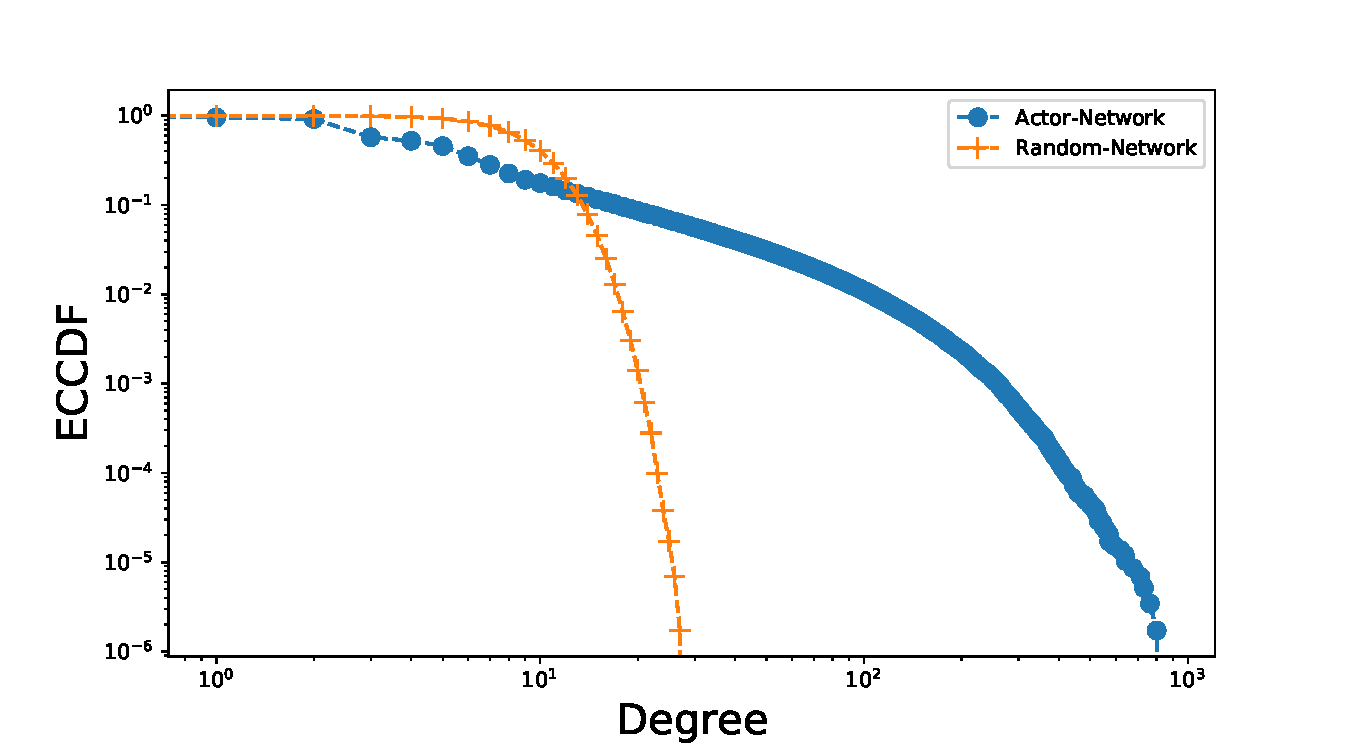
\includegraphics[width=\textwidth]{degree-distribution.pdf}
    \caption{ECCDF (Empirical Complementary Cumulative Distribution Function) of the degree distribution of the actor co-partecipation network (blue) and that of Erdős–Rényi's equivalent random network (orange) in log-log scale.}
    \label{fig:degree-distribution}
\end{figure}

\section{Algorithms}
\label{sec:algorithms}

\subsection{Degree}
\label{degree}
In an undirected unweighted graph the degree of a node is basically the number of edges incident to it. In our case we have a directed graph so we can distinguish between indegree and outdegree. The indegree of a node $i$ is the number of links having target equal to $i$ while the outdegree is the number of links having source equal to $i$. The indegree is typically a measure of influence of the node while the outdegree is a measure of expansiveness. For this reason I have chosen to use indegree as a first system ranking nodes. In the class \textit{ActorGraph} there is a field \textit{out\_degree} and as described in \ref{graph-construction} in our case is equivalent to an indegree dictionary so we can easily return that attribute to compute the indegree of the nodes. The computational cost of this operation is $\mathcal{O}(1)$ but It requires $\mathcal{O}(|V|)$ space.


\subsection{PageRank}
\label{pagerank}
PageRank computes a ranking of the nodes in the graph $G$ based on the structure of the incoming links. It was originally designed as an algorithm to rank web pages. According to Google, PageRank works by counting the number and quality of links to a page to determine a rough estimate of how important the website is. The underlying assumption is that more important websites are likely to receive more links from other websites \footnote{\url{https://web.archive.org/web/20111104131332/https://www.google.com/competition/howgooglesearchworks.html}, September 2021 \label{google}}. \\PageRank can be easily used to compute ranking on any type of directed graph. For each node $i$ there is an associated PageRank $q_{i}$ which measures the importance of node $i$. The PageRank is a number between 0 and 1; the bigger the PageRank, the more important the page. The vector $q$ of all Pageranks is a probability distribution, that is, the PageRanks sum to one. There is not one fixed algorithm for assignment of PageRank, and in fact variations on the basic idea can alter the relative PageRank of any two pages. \\
I have implemented my PageRank using the power iteration method as generally described in the book by Leskovec, Rajaraman and Ullman \cite{leskovec2014}. I recall that $q$ can be computed by multiplying:
\[ q = M^j \cdot p \]
where $M$ is a $|V| \times |V|$ matrix that represents the structure of the graph, $p$ is a vector of $|V|$ elements that describes the distribution of PageRank already setted or computed and $j$ is the number of iterations. Usually $p$ is initialized to the uniform probability, that is $p = [\frac{1}{|V|}]_{1,...,|V|}$. The method stops when the difference in a certain convergence measure (e.g. l1 norm) between the pagerank at step $j$ and the pagerank at step $j-1$ is less than a fixed threshold $\epsilon$. Tipically are necessary up to one hundred iterations to allow PageRank to converge with big graphs \cite{leskovec2014}. \\
To describe how I computed a single step I need to specify how $M$ is constructed. $M$ has 3 components:
\begin{equation}
\label{eq:M}
    M = \beta \cdot A + \beta \cdot D + (1 - \beta) \cdot T
\end{equation}
$\beta$ is a number between 0 and 1 representing the probability of selecting an outgoing link, $(1-\beta)$ is the probability of teleporting. Usually $\beta$ is setted to 0.85 \cite{leskovec2014}. $A$ is the transition matrix of the graph and the cell $A_{ij}$ is equal to zero if the node $j$ has no link to $i$ and $\frac{1}{d^{\mathrm{out}}_{j}}$ otherwise, where $d^{\mathrm{out}}_{j}$ is the outdegree of node $j$. Note that $A$ is a very sparse matrix and I don't need to store it as it is: in fact, I've implemented a data structure in class \textit{ActorGraph} that allows to store transition matrix in a more compact way as generally described in Chapter 5.2.1 of \cite{leskovec2014}. $D$ is the dangling matrix in which the column $j$ is equal to $\frac{1}{|V|}$ in all its entries if $j$ is a dangling node and zero otherwise. Also $D$ is very sparse and we can easily store only a boolean vector $d$ of dangling nodes. $T$ is the teleporting matrix and It has all its entries equal to $\frac{1}{|V|}$ so we need to store just a number.\\
By using Eq. \ref{eq:M} I computed for each node $i$ the products $(A \cdot p)_{i}$, $(D \cdot p)_{i}$, $(T \cdot p)_{i}$ separately and then I summed them with the factors $\beta$ or $(1-\beta)$. In this way there is the need to store in main memory only vectors of dimension $|V|$.

\subsubsection{Time and Space Complexity}
To compute $(T \cdot p)_{i}$ for a node $i$ I multiplied $(1-\beta)\cdot \frac{1}{|V|}$ and it requires $\mathcal{O}(1)$ space and operations. I computed the dangling contribution only one for each step and it is equal to $\mathbf{1}\cdot(d\cdot p)/n$ so it requires $\mathcal{O}(|V|)$ operations and space. To compute $(A \cdot p)_{i}$ for a node $i$ I executed $(A \cdot p)_{i} = \sum_{k} A_{ik}\cdot p_{k}$ so, thanks to the data structure implemented in class \textit{ActorGraph}, the total number of operations on the overall nodes of the graph is upperbounded by $|E|$. The theoretical complexity of my PageRank is $\mathcal{O}(j(|V| + |E|))$ and it requires $\mathcal{O}(|V|)$ space where $j$ is the number of iterations. Note that $|E|$ typically grows more than linearly w.r.t. the number of nodes but much slower than $|V|^{2}$ \cite{densification} so there is a great saving in terms of both space and operations compared to using matrices.

\subsubsection{Empirical performance evaluation}

I also evaluated through some experiments the performance of my PageRank compared to the performance of the simplest PageRank implementation in Networkx, maybe the most used Python package for network analysis.\\ Figure \ref{fig:performance} shows the execution time of the two implementations of PageRank in function of the number of nodes  and density in random graphs. Both plots show that my implementation is faster than the one provided by NetworkX and this result makes it an acceptable implementation. \\ To construct different random graphs with different number of nodes I used the Barabási–Albert model \cite{Albert2002}, a model that shows properties very similar to real scale free networks such as my net, implemented in Networkx. To construct different random graphs with different density (probability to find a link between two nodes) I used the Erdős–Rényi model that allows to specify easily this parameter. \\ For the experiments showed in Figure \ref{fig:performance}a I used number of nodes \{$1\cdot10^{3}, 1\cdot10^{4}, 5\cdot10^{4}, 1\cdot10^{5}, 2\cdot10^{5}, 3.5\cdot10^{5}, 5\cdot10^{5}$\}, the default values for \textit{barabasi\_albert\_graph} method except for the number of nodes and for number of edges to attach from a new node to existing nodes (setted to nine because is the avg. degree of our graph as showed in Tab. \ref{tab:graph-property}), the default values for Networkx and my PageRank except for tollerance threshold ($\epsilon$) setted to 0.01. \\For the experiments showed in Figure \ref{fig:performance}b I used densities \{$1\cdot10^{-6}$, $1\cdot10^{-5}$, $1\cdot10^{-4}$, $2.5\cdot10^{-4}$, $5\cdot10^{-4}$, $7.5\cdot10^{-4}$, $1\cdot10^{-3}$\}, $N$ equal to $10^{5}$ for \textit{fast\_gnp\_random\_graph} method, the same values of the experiments mentioned above for the rest. I have not considered values above $1\cdot10^{-3}$ for density because real networks are very sparse so It is not relevant.\\ All experiments were executed 3 times to increase reliability of the results.
\begin{figure}
     \centering
     \begin{subfigure}{0.45\textwidth}
         \centering
         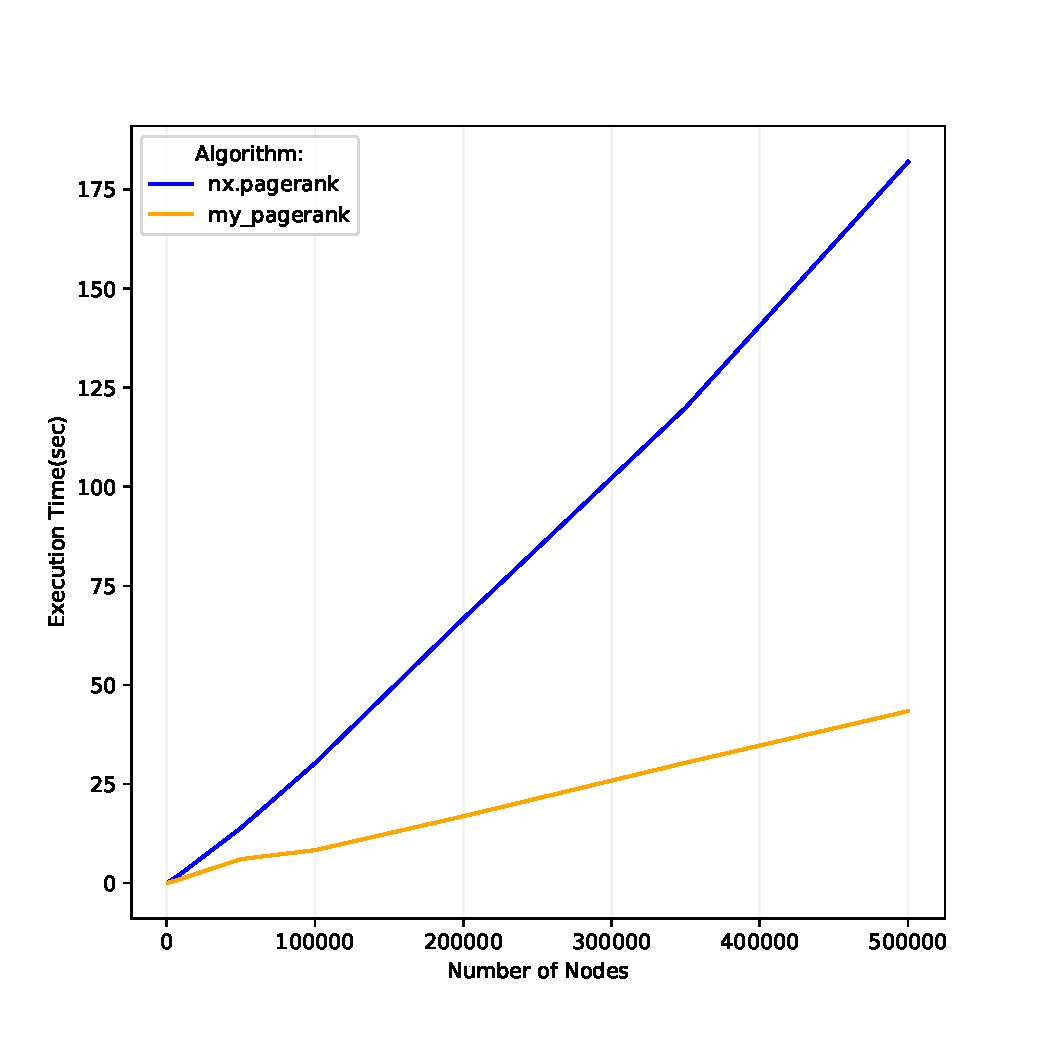
\includegraphics[width=\textwidth]{time_for_nodes.pdf}
         \subcaption[]{}
         \label{fig:times_for_nodes}
     \end{subfigure}
     \hfill
     \begin{subfigure}{0.45\textwidth}
         \centering
         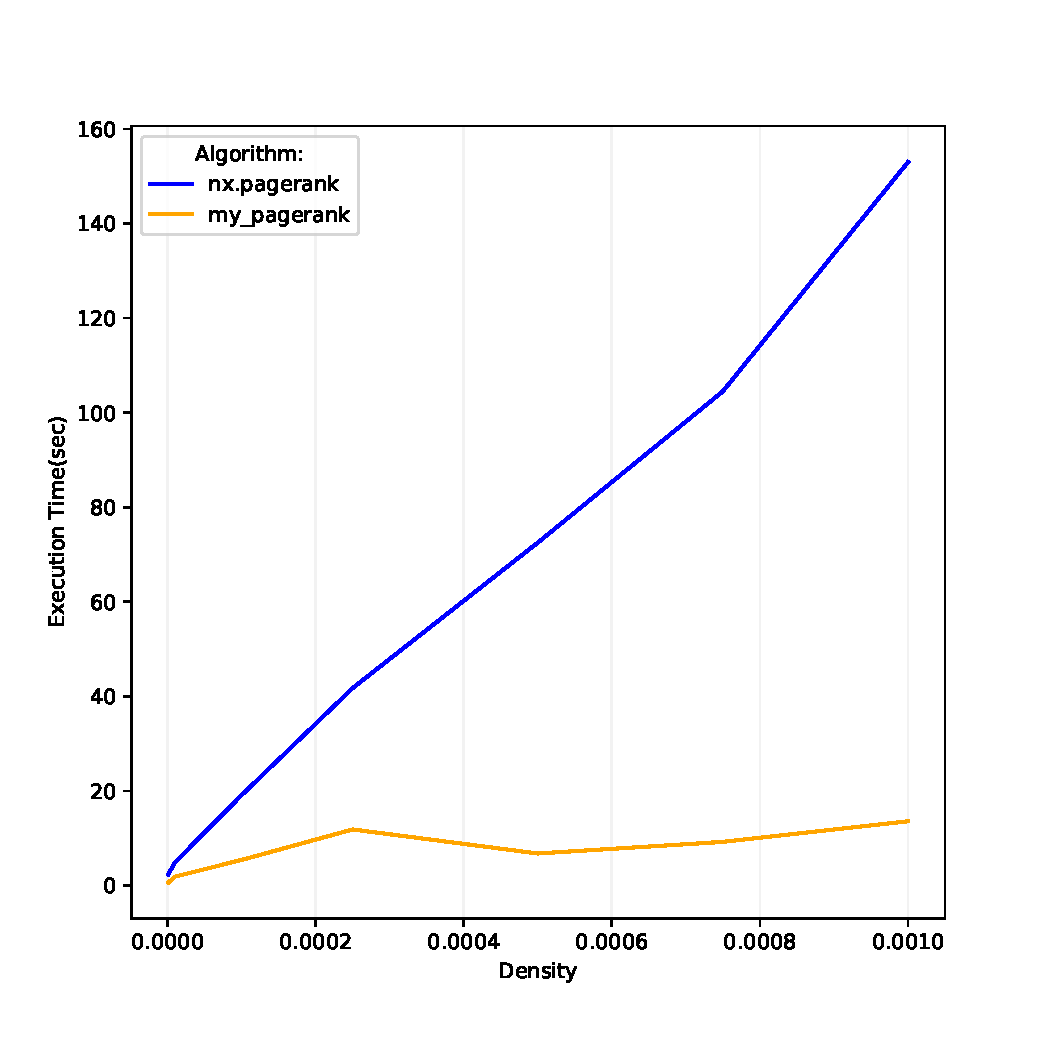
\includegraphics[width=\textwidth]{time_for_density.pdf}
         \subcaption[]{}
         \label{fig:times_for_density}
     \end{subfigure}
     \hfill
    \caption{\textbf{(a)} Execution time (in seconds) of Networkx (blue) and my Pagerank (orange) implementation in function of number of nodes in Barabási–Albert graphs. \textbf{(b)} Execution time (in seconds) of Networkx (blue) and my Pagerank (orange) implementation in function of density in Erdős–Rényi graphs.}
    \label{fig:performance}
\end{figure}

\subsubsection{Empirical convergence evaluation}
Figure \ref{fig:convergence} shows the convergence rate with different convergence measure for one hundred iterations of my PageRank implemention on the actor co-partecipation network. For these experiments I used the default values of the method. 
I chose to use l1-norm as default convergence measure because that is the choice of Networkx implementations and I decided to present also l2-norm because is the measure we saw during the course and the max absolute difference between 2 elements of the vectors, that is $\max_{j} |(M\cdot p - p)_{j}|$, because is an alternative different way to measure the convergence. The plot shows that after one hundred iterations the convergence rates are very small but for l1 and l2-norm there is no convergence while for max absolute difference there is more stable rate after 80 iterations. This result tells that max absolute difference is less conservative but more relevant measure. The plot can be used also to choice a good configuration for $\epsilon$ and \textit{max\_iter} parameters. \\ In Figure \ref{fig:toy-convergence} I also plotted the convergence rates on a toy example of few nodes and links that shows rates reach zero with smaller graphs. Note that all the systems ranking nodes have been tested on toy examples that are visible on github.
\begin{figure}
    \centering
    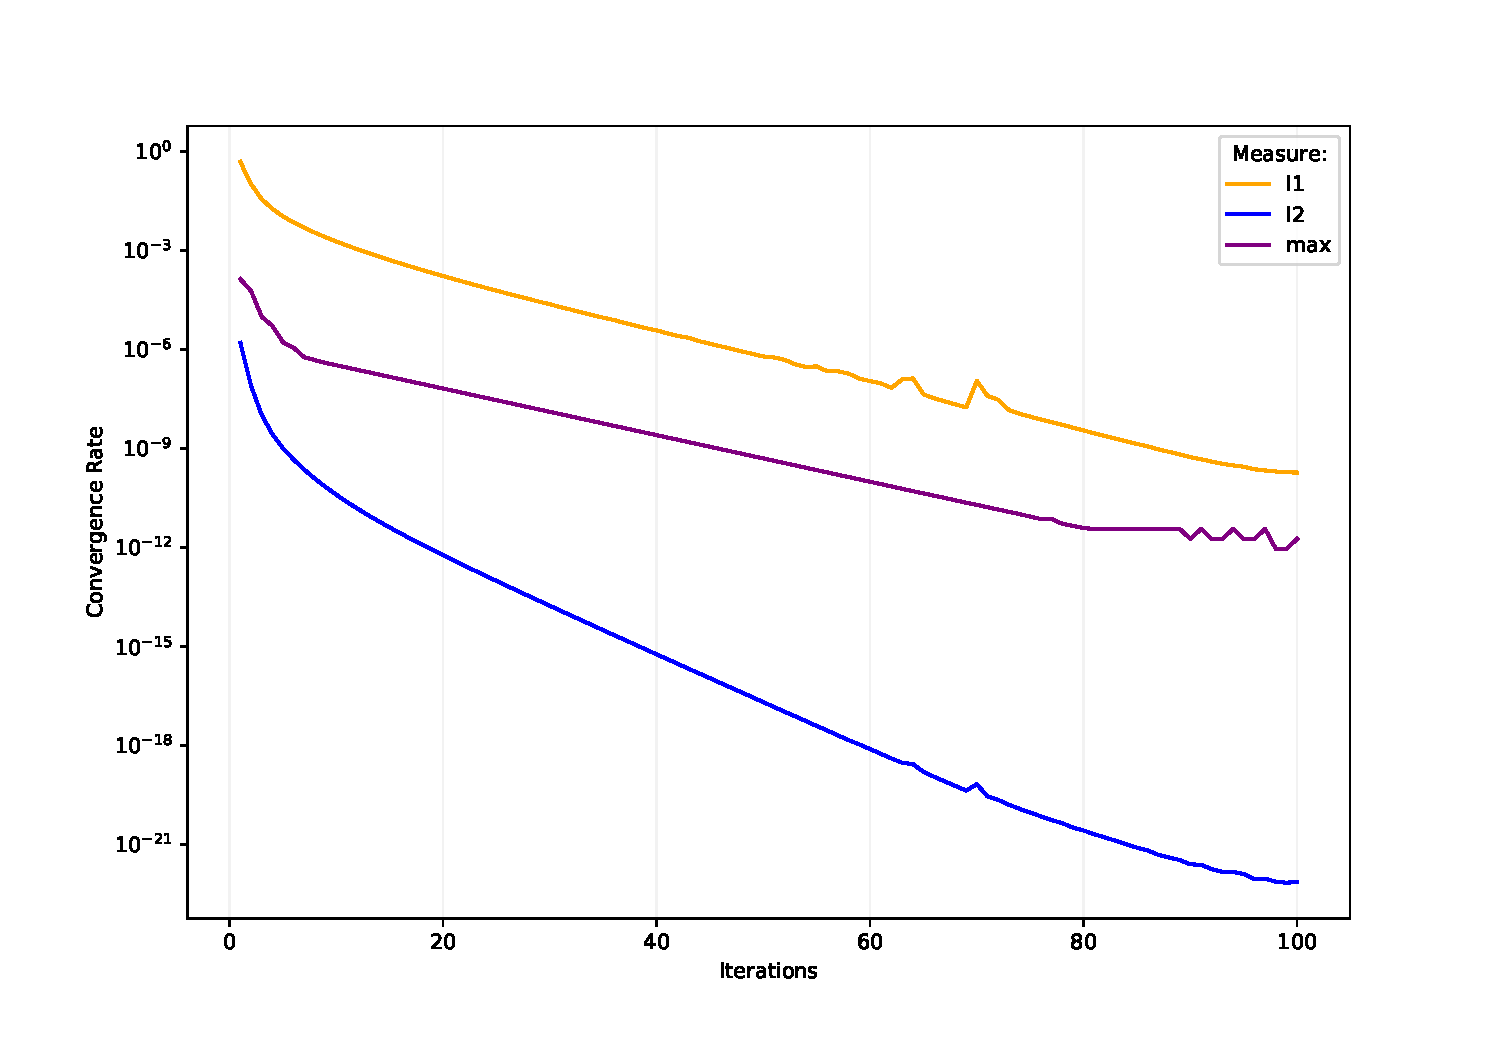
\includegraphics[width=\textwidth]{convergence_per_iteration.pdf}
    \caption{Convergence rate in function of PageRank iterations with l1-norm (orange), l2-norm (blue), max absolute difference between 2 elements (purple) on actor co-partecipation network.}
    \label{fig:convergence}
\end{figure}

\begin{figure}
    \centering
    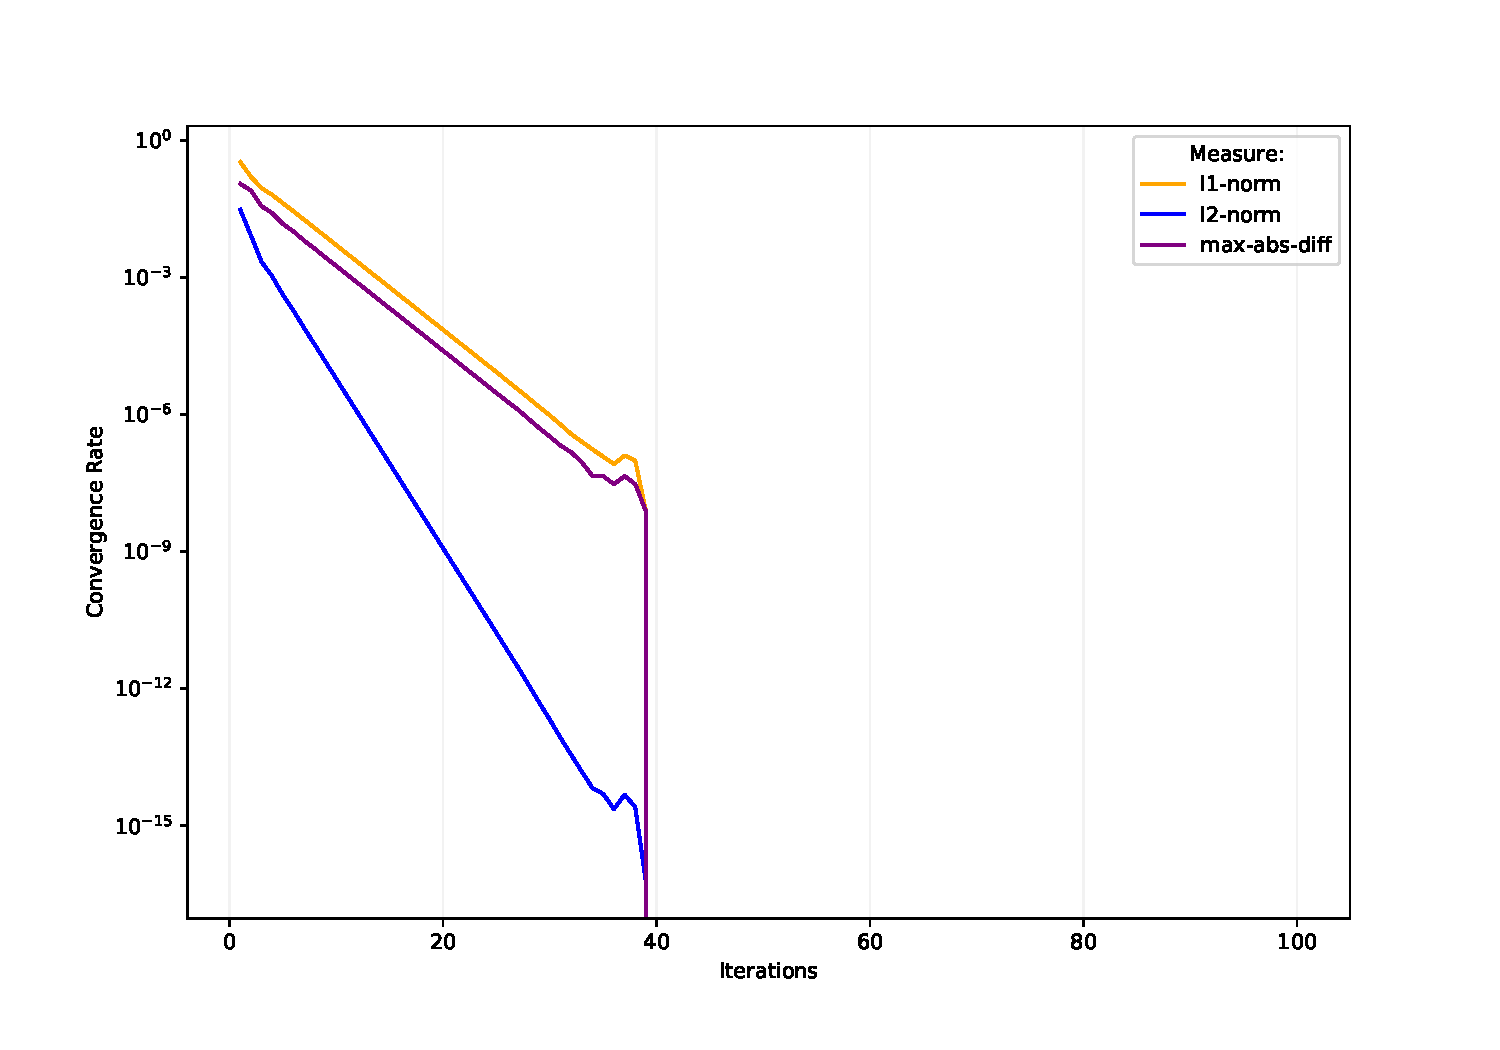
\includegraphics[width=0.9\textwidth]{toy_convergence_per_iteration.pdf}
    \caption{Convergence rate in function of PageRank iterations with l1-norm (orange), l2-norm (blue), max absolute difference between 2 elements (purple) on toy example.}
    \label{fig:toy-convergence}
\end{figure}

\subsubsection{Topic-Sensitive PageRank}
Topic-Sensitive PageRank is a modification of PageRank in which the teleporting is not to any other node but only to certain nodes. The teleporting from node $i$ to node $j$ is allowed only if $i$ and $j$ are classified with the same fixed topic $t$. Suppose you have a vector $s$ that represents a teleporting set in which the $i$-th component is equal to 1 if node $i$ is classified with $t$ and zero otherwise. Then the teleporting contribution is equal to $[(1-\beta)\cdot\frac{1}{|s|}\cdot s]$ instead of $[(1-\beta)\cdot\frac{1}{|V|}\cdot\mathbf{1}]$ for PageRank.\\
The idea behind Topic-Sensitive PageRank is, for example in the context of Web Pages, to build different rankings according to different topics assigned to pages and extracted from queries or user preferences to order the results in more sophisticated way w.r.t. single PageRank. I used \textit{genderAttribute} dictionary in class \textit{ActorGraph} to build a Topic-Sensitive Page Rank for actor co-partecipation network. Performance and convergence analysis can be easily extended to this version of PageRank.

\subsection{HITS}
\label{hits}
HITS (Hyperlink-Induced Topic Search) is know as the hub and authority approach for ranking nodes. Given a directed unweighted graph, an hub is a node that is a source of edges to good authority nodes while an authority is a node that is the target of edges from good hub nodes. Note that in actor co-partecipation network the concepts of hub and authority coincide because the network is semantically undirected.\\
I implemented HITS, using the same data structure for graph informations used for PageRank, that performs the following steps:
\begin{enumerate}
    \item Inizialization of hub and authority score of each node to one.
    \item Authority update: update each node's authority score to be equal to the sum of the hub scores of each node that points to it.
    \item Hub update: Update each node's hub score to be equal to the sum of the authority scores of each node that it points to.
    \item Normalization of the values by dividing each hub score by the sum of all hub scores, and dividing each authority score by the sum of all authority scores.
    \item Repetition from step 2 to 4 for a certain number of iterations $j$.
\end{enumerate}
It's easy to understand that the number of operations in a single step of HITS is dominated by the update rule and it requires $\mathcal{O}(|E|)$ operations so the time complexity of HITS is $\mathcal{O}(j\cdot |E|)$ where $j$ is the number of iterations.\\
HITS, like PageRank, is an iterative algorithm based on linkage of the nodes for ranking them. However it does have some major differences respect to PageRank:
\begin{itemize}
    \item It computes two scores per node, hub and authority, as opposed to a single score.
    \item It requires less execution time.
    \item In the context of search engines, It is tipically computed on a subgraph of interest (obtained from a certain query) at query time instead of on the whole graph at batch time.
\end{itemize}


\section{Experiments}
\label{sec:experiments}
\subsection{Ranking comparison}
Table \ref{tab:rankings} resumes the top 10 actors and actresses for each centrality index. PageRank and the Topic-Sensitive version were computed with the default values for parameters while HITS was computed for 60 iterations. \\In all the rankings there are actors from the pornographic industry and from Indian cinema where co-participation is typically high as well as collaborations between famous actors in the sector. \\ Degree centrality simply returns the top 10 nodes that have achieved the most co-participations: in fact at the first place there is Brahmanandam that currently holds the Guinness World Record for the most screen credits for a living actor. \\ PageRanks tends to give more importance to nodes that are connected to important nodes: Eric Roberts is an american actor that has received two nominations at Golden Globe and even if he has less credits than Brahmanandam he is more internationally known. Topic-Sensitive PageRank changes the ranking thanks to the bias introduced in teleporting but not in the expected way: It does not introduce any actresses into the top 10, probably because the teleporting set linked to female gender is too big to have a noticeable impact. \\ The authority score produces very different results from the other centrality measures considered because I think it accounts differently the local structures of the network compared to the global one.
\begin{table}[]
    \centering
    \begin{adjustbox}{max width=\textwidth}
    \begin{tabular}{c|c|c|c|c}
    Ranking &   In-Degree &     PageRank &      Ts-PageRank &       HITS-Auth  \\
    \hline
    1 &     Brahmanandam &      Eric Roberts &  Eric Roberts &      Aruna Irani \\
    2 &     Ron Jeremy &        Brahmanandam &      Masayoshi Nogami &      	Helen \\
    3 &     Eddie Garcia &      Masayoshi Nogami &      Ron Jeremy &        Ashok Kumar \\
    4 &     Eric Roberts &      Ron Jeremy &        Seiji Nakamitsu &       Master Bhagwan \\
    5 &     Masayoshi Nogami &      Joe Estevez &       Brahmanandam &      Pran \\
    6 &     Paquito Diaz &      Michael Madsen &        Kôji Makimura &         Dharmendra \\
    7 &     Mithun Chakraborty &        Tom Sizemore &      Yutaka Ikejima &        Jagdeep \\
    8 &     Shakti Kapoor &     Seiji Nakamitsu &       Tom Byron &     Jeevan \\
    9 &     Tom Byron &     Tony Devon &        Jamie Gillis &      Mohan Choti \\
    10 &    Aruna Irani &       Danny Trejo &       Jean-Pierre Armand &        Madan Puri \\	
    \end{tabular}
    \end{adjustbox}
    \caption{Top 10 nodes for Degree, PageRank, Topic-Sensitive PageRank, HITS centrality.}
    \label{tab:rankings}
\end{table}

\subsection{Top 10 IMDB similarity}
I compared the results of the centrality measures on a subset of nodes of interest. This subset is the top 10 actors and actresses of all time by IMBD. I also considered the results of the harmonic centrality \footnote{I used networkx 2.5 to compute harmonic centrality, the implementation of this algorithm is changed in version 2.6 released on July and adopted by Colab in mid-August.} because is an interesting index as is the only centrality measure that pass the axioms for centrality proposed by Boldi and Vigna \cite{Boldi2013}. To do this, I did the following steps:
\begin{enumerate}
    \item I computed the centrality measure on the whole graph and I filtered the results only on the nodes of interest obtaining the ranking on the top 10 of all time for each system ranking nodes.
    \item I computed the similarity between each pair of rankings using a similarity measure.
    \item I constructed the similarity matrix between rankings.
\end{enumerate}
I used two different similarity measures: the Hamming similarity, that is one minus the Hamming distance \cite{Hamming1950} (simply the number of different positions in the two rankings) and the Kendall Tau distance \cite{Hamming}, a measure of the correspondence between two rankings that is equivalent to the number of bubble sort steps to pass from one ranking to the other.\\
Figure \ref{fig:similarity} shows the heatmaps of the similarity matrices between top 10 of all time rankings considering Hamming and Kendall Tau similarity. The Hamming matrix shows very low similarities due to the fact that the measure is very simple and not designed for ranking but It tells us that the most interesting centrality measure for top 10 of all time are authority score and harmonic centrality. The Kendall Tau matrix confirms what is described by the Hamming one but shows higher similarity values. In particular, harmonic centrality and authority score have similarity with IMBD ranking close to 0.5 and they seem to be able to capture in some way the popularity of actors. \\ The matrix is also useful to have an idea on the difference between the centrality measures: for example, degree is more similar to harmonic centrality than to PageRank because the first two are both geometric measure (measures assuming that importance is a function of distances) while PageRank is a spectral measure (it computes the left dominant eigenvector of some matrix derived from the graph).
\begin{figure}
     \centering
     \begin{subfigure}{0.49\textwidth}
         \centering
         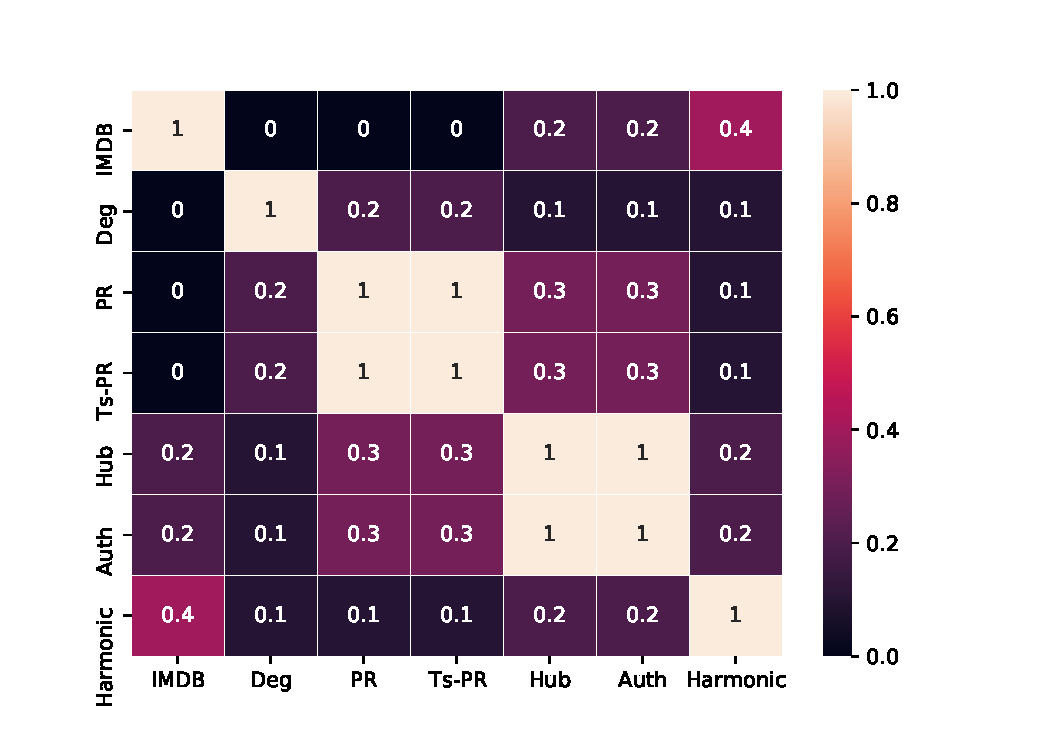
\includegraphics[width=\textwidth]{hamming-heatmap.pdf}
         \subcaption[]{}
         \label{fig:hamming}
     \end{subfigure}
     \hfill
     \begin{subfigure}{0.49\textwidth}
         \centering
         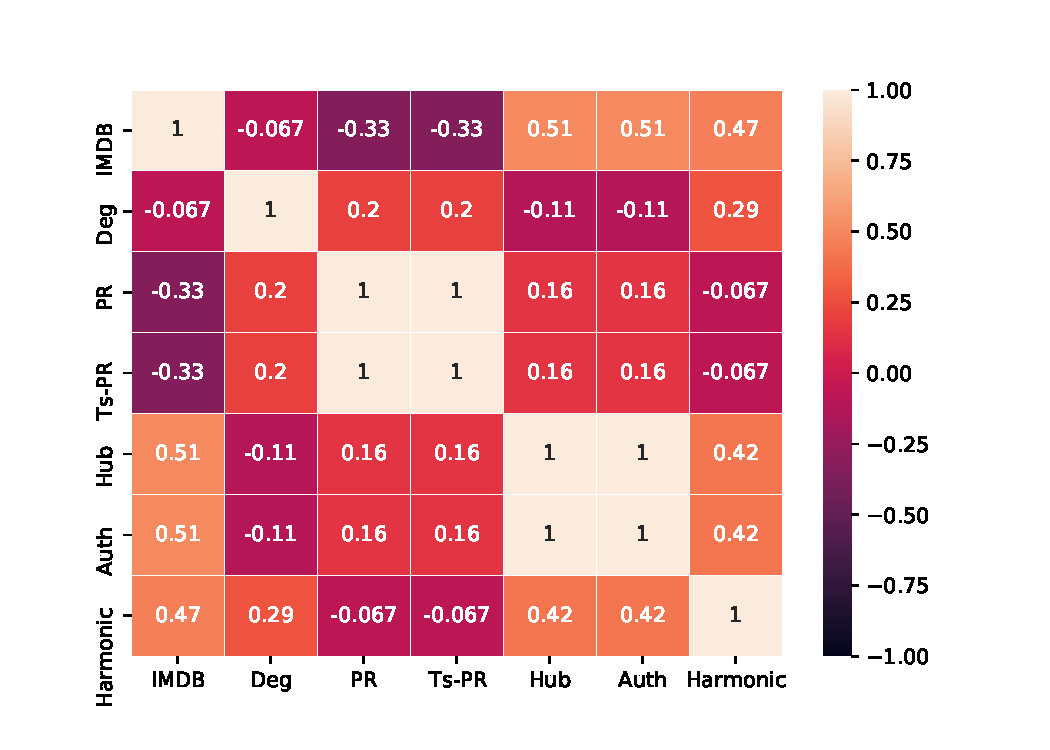
\includegraphics[width=\textwidth]{kendalltau-heatmap.pdf}
         \subcaption[]{}
         \label{fig:kendalltau}
     \end{subfigure}
     \hfill
    \caption{\textbf{(a)} Heatmap of the similarity matrix between top10 of all time rankings using Hamming similarity. \textbf{(b)} Heatmap of the similarity matrix between top 10 of all time rankings using Kendall Tau similarity.}
    \label{fig:similarity}
\end{figure}

\section*{Conclusion}
This report describes the implementation, efficiency and results of systems ranking nodes in a directed unweighted graph. The graph considered is an actor co-partecipation graph obtained from the IMDB dataset in which nodes identify actors and edge links two nodes if the corresponding actors played at least once in the same movie. This network is a sparse and scale free network. My PageRank implementation, thanks to an efficient representation of the graph, is competitive with the implementations provided by Networkx. An empirical evaluation on PageRank tells that the max absolute difference is a relevant measure for convergence. HITS, and in particular the authority score, seems to be able to capture in some way the popularity of actors because it produces the most similar ranking to the top 10 actors and actresses of all time provided by IMDB.

\bibliography{biblio}{}
\bibliographystyle{unsrt}
\addcontentsline{toc}{chapter}{References}

\end{document}
